%  $Description: Author guidelines and sample document in LaTeX 2.09$
%  $Author: ienne $
%  $Date: 1995/09/15 15:20:59 $
%  $Revision: 1.4 $
%\documentstyle[times,art10,twocolumn,latex8]{article}
%-------------------------------------------------------------------------
% take the % away on next line to produce the final camera-ready version
%-------------------------------------------------------------------------


\documentclass[times,10pt,twocolumn]{article}
%%%%%%%%%%%%%%%%%%%%%%%%%%%%%%%%%%%%%%%%%%%%%%%%%%%%%%%%%%%%%%%%%%%%%%%%%%%%%%%%%%%%%%%%%%%%%%%%%%%%%%%%%%%%%%%%%%%%%%%%%%%%%%%%%%%%%%%%%%%%%%%%%%%%%%%%%%%%%%%%%%%%%%%%%%%%%%%%%%%%%%%%%%%%%%%%%%%%%%%%%%%%%%%%%%%%%%%%%%%%%%%%%%%%%%%%%%%%%%%%%%%%%%%%%%%%
\usepackage{latex8}
\usepackage{times}
\usepackage{graphicx}

\pagestyle{empty}

\begin{document}

\title{Solving System of Linear Equations in a Network of Workstations}
\author{Gabriel Dimitriu \\
%EndAName
"Politehnica" University of Bucharest\\
Splaiul Independentei nr313,060042,Romania\\
gabriel@tech.pub.ro\\
\and Felicia Ionescu \\
%EndAName
"Politehnica" University of Bucharest\\
Splaiul Independentei nr313,060042,Romania\\
 fionescu@tech.pub.ro
}
\maketitle

\begin{abstract}
In this article we propose an evaluation of the three common algorithms 
for solving linear system of equations: Gauss Elimination, Gauss-Jordan 
without pivoting and Jacobi with dominant rows. The parallel design of 
the chosen algorithms is a compromise between the easies and elegant 
way to implement in MPI and the performance. The result confirmed that 
for a small number of low cost computers the speedup is acceptable for 
the Gauss Elimination and Gauss-Jordan but for Jacobi with dominant rows 
if data is not already distributed is better to implement the serial version.
\end{abstract}

\thispagestyle{empty}

%-------------------------------------------------------------------------
\Section{Introduction}

In recent years, networks of workstations (NOWs) and clusters of
workstations (COWs) have become the fastest growing choice for
building parallel platforms. The success of clusters and NOWs has
been mainly facilitated by the rapid advancement of microprocessor
technologies and high-speed network interconnects, such as Myrinet
and Giganet. The increased accessibility and relatively low cost
of these technologies are also important factors for the wide
acceptance of clusters among users. For NOWs, the most important
factor is very low cost, we can use old network of PCs which
normally is used in laboratory, or inside corporation, for high
performance computing during night, or days off or any time these
computers are not used. Typically a NOWs is made from a number of
PCs which have LINUX as operating system and MPI or PVM as a
parallel computing library. We will present some high and low
computational algorithms for solving a system of linear equations.


%-------------------------------------------------------------------------
\Section{Background}

Let be \begin{equation}AX=B\label{s1}\end{equation} our system of
linear equations. Where A is a dense square matrix with dimension
n, and let be $A[i][j]=a{_i}{_j}$ his elements. The solution of
the system (X) is a vector with dimension n with $x_i$ as
components. The free term (B) is a vector with n dimension with
$b_i$ as components.

This system could be solved using one of the following methods:
Gaussian Elimination, Gauss-Jordan or Crout if we don't have
another information about the matrix A; Jacobi or Gauss-Siedel if
the matrix is column or row dominant.


%-------------------------------------------------------------------------
\SubSection{Gaussian Elimination}

The system of equations is solved in two stages. First, through a
series of algebraic manipulations, the original system of
equations is reduced to an upper triangular system of the form
$U*X=Y$, where U is a unit upper-triangular matrix. In the second
stage of solving a system of linear equations, the
upper-triangular system is solved for the variables in reverse
order from $x_{n-1}$ to $x_0$ by a procedure know as
back-substitution.

\begin{enumerate}
\item procedure gaussian\_elimination(A,b,y)
\item begin
\item for k:=0 to n-1 do
\item for j:=k+1 to n-1 do
\item A[k][j]:=A[k][j]/A[k][k]; //division step
\item y[k]:=b[k]/A[k][k];
\item A[k][k]:=1;
\item for i:=k+1 to n-1 do
\item for j:=k+1 to n-1 do
\item A[i][j]:=A[i][j]-A[i]k]*A[k][j]; //elimination step
\item b[i]:=b[i]-A[i][k]*y[k];
\item A[i][k]:=0;
\item endfor;
\item endfor;
\item end\_procedure gaussian\_elimination;
\end{enumerate}

%-------------------------------------------------------------------------
\SubSection{Gauss-Jordan}

Through a series of algebraic manipulations, the attached matrix
of the linear system is reduced to a unity matrix so the system is
$I*X=Y$.

\begin{enumerate}
\item procedure gauss\_jordan(A,b,x)
\item begin
\item for k:=0 to n-1 do
\item for i:=0 to n-1 do
\item if(k $< >$ i) then do
\item for j:=k+1 to n-1 do
\item A[i][j]-=A[i][k]/A[k][k]*A[k][j];
\item endfor;
\item b[i]-=A[i][k]/A[k][k]*b[k];
\item endif;
\item endfor;
\item endfor;
\item for i:=0 to n-1 do
\item x[i]=b[i]/A[i][i];
\item endfor;
\item end\_procedure gauss\_jordan;
\end{enumerate}

%-------------------------------------------------------------------------
\SubSection{Jacobi with dominant rows}

 Suppose $a_{ii}\not=0$ for any $i\in\{1\ldots ,n\}$ then we can note
\begin{displaymath}
 D=\left(\begin{array}{ccc}
a_{11} & \ldots &0 \\
\ddots &\ldots &\ddots \\
 0 & \ldots & a_{nn}
\end{array}\right)
\end{displaymath}

and

\begin{displaymath} D^{-1}=\left(\begin{array}{ccc}
 1/a_{11} &\ldots &0\\
\ddots & \ldots &\ddots \\
0 & \ldots & 1/a_{nn}
\end{array}\right)
\end{displaymath}

 The system (\ref{s1}) could be transform in $D^{-1}*A*X=D^{-1}*B$ or
$$(I-(I-D^{-1}*A))X=D^{-1}*B$$
 which is equivalent with
    \begin{equation}(I-C)x=B \label{s2}\end{equation}

{\bf Jacobi Theorem}

If
\begin{equation}
|a_{ii}|>\sum_{j=1,j\not=i}^{n}|a_{ij}|,\forall
i\in{1,...,n}\label{jaccond}
\end{equation}

then the system (\ref{s2}) has the unique solution z and $\forall
x^{(0)}\in R^m$ the string $(x^{(n)})_{n\in N}$ with
$x^{(n+1)}=C*x^{(n)}+B$ convert to z and it takes places the
following relations:

$$\|x^{(n)}-z\|_{\infty}\le\frac{q}{1-q}\|x^{(n)}-x^{(n-1)}\|_{\infty}$$
where
\begin{equation}
q=\max_{1\le i\le n}\sum_{j=1,j\ne i}^{n}\left |\frac{a_{ij}}{a_{ii}}\right |\label{q}
\end{equation}
and
\begin{equation}
\|x\|_\infty=\max_{1\le i\le n}|x_i|\label{norma}
\end{equation}

%------------------------------------------------------------------------
\Section{Design of the parallel algorithms}

Because in such type of problems we want to obtain a high speedup
defined by $\frac{Serial\; time}{Parallel\; time}$ first we have
to check if the distribution of data over network isn't close to
the serial time of the chosen problem. This must be check because
the time difference in absolute value between the distribution
time and serial time divided by the number of machines is the
maximum time required for the parallel execution to obtain the
speedup equal to the number of machines.

For the Gauss and Gauss-Jordan the matrix and free term will be 
distributed among machines using a cyclical striped row type.
So the processors are arranged in a cyclical queue and each two 
consecutive lines are distributed among two consecutive machines.
Suppose the matrix has n rows and we have p machines. Then a
machine k has the following rows: \{k,k+p,k+2p,\ldots \}. So any
machine with MPI-rank k will have the rows who correspond to the
following relation $row=k+r*p$ with $r\in \{0,1,\ldots ,n/p+1\}$.

%-------------------------------------------------------------------------
\SubSection{Gaussian Elimination}

During the $k^{th}$ iteration processor $P_{k}$ broadcast part of
the $k^{th}$ row of the matrix to processors $P_{k+1}\ldots
P_{p-1}$. Assume that the processors $P_0\ldots P_{p-1}$ are
connected in a linear array, and $P_{k+1}$ is the first processor
to receive the $k^{th}$ row from processor $P_{k}$. Then the
processor $P_{k+1}$ must forward this data to $P_{k+2}$. However,
after forwarding the $k^{th}$ row to $P_{k+2}$, processor
$P_{k+1}$ need not wait to perform the elimination step until all
the processors up to $P_{p-1}$ have received the $k^{th}$ row.
Similarly, $P_{k+2}$ can start it's computation as soon as is has
forwarded the $k^{th}$ row to $P_{k+3}$, and so on. Meanwhile,
after completing the computation for the $k^{th}$ iteration,
$P_{k+1}$ can perform the division step, and start the broadcast
of the $(k+1)^{th}$ row by sending it to $P_{k+2}$.

We chose for this algorithm the pipeline approach, presented in
\cite{kumar}, and with matrix and free term scaterred with cyclic
striped row strategy. These facts conduct to the following
behavior of the each machine:
\begin{enumerate}
\item If the machine has any data destined for other machine, it
send those data to the appropriate processor.
\item If the machine can perform some computation, it does.
\item Otherwise, the machine waits to receive data from other
machines.
\end{enumerate}

\begin{figure}[h]
   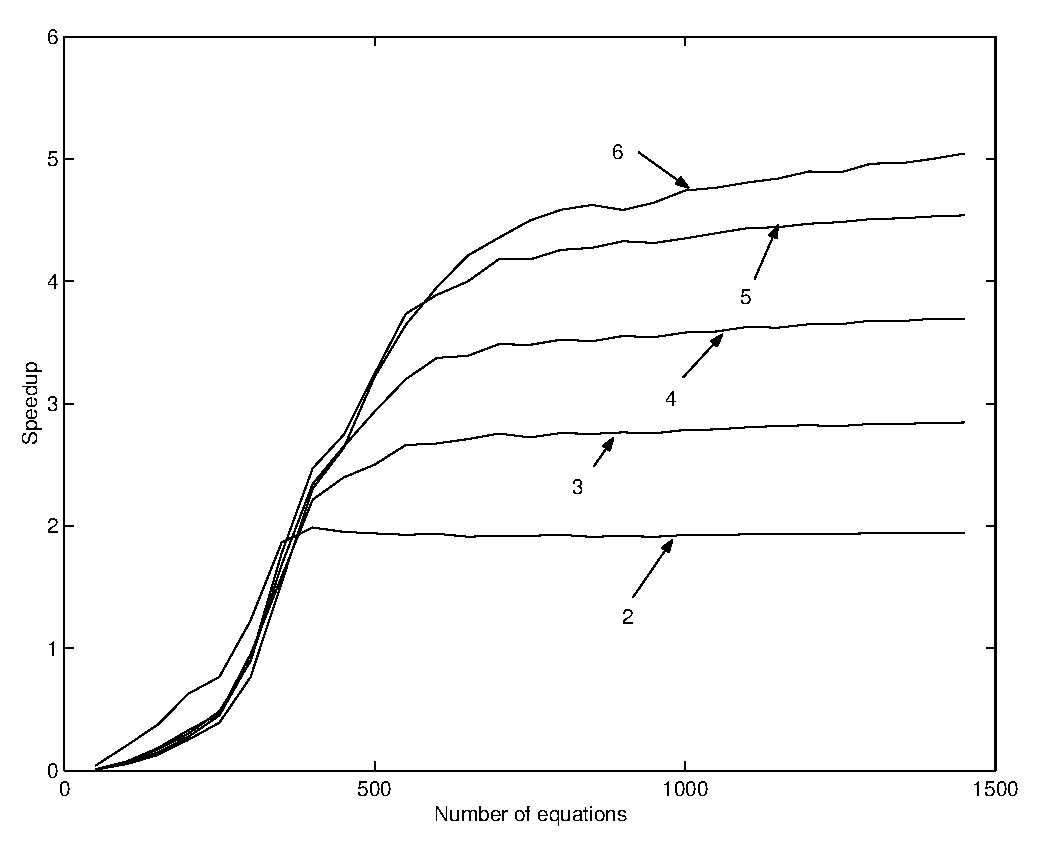
\includegraphics[scale=0.44]{ge-mpich2-bw.eps}
   \caption{Gaussian Elimination Speedup}
\end{figure}

%-------------------------------------------------------------------------
\SubSection{Gauss-Jordan}

During the $k^{th}$ iteration processor $P_{k}$ broadcast the
$k^{th}$ row of the matrix to processors all processors. Assume
that the processors $P_0\ldots P_{p-1}$ are connected in a linear
array, and $P_{k+1}$ is the first processor to receive the
$k^{th}$ row from processor $P_{k}$. Then the processor $P_{k+1}$
must forward this data to $P_{k+2}$. However, after forwarding the
$k^{th}$ row to $P_{k+2}$, processor $P_{k+1}$ need not wait to
perform the lines from 4 to 11 of the algorithm for it's part of
matrix until all the processors up to $P_{p-1}$ have received the
$k^{th}$ row. Similarly, $P_{k+2}$ can start its computation as
soon as is has forwarded the $k^{th}$ row to $P_{k+3}$, and so on.
Meanwhile, after completing the computation for the $k^{th}$
iteration, $P_{k+1}$ start the broadcast of the $(k+1)^{th}$ row
by sending it to $P_{k+2}$. All processors receive $p-1$ rows
before sending their rows to other processors.

We chose for this algorithm the pipeline approach and with matrix
and free term scaterred with cyclic striped row strategy. These
facts conduct to the same  behavior as Gauss Elimination.

\begin{figure}[h]
   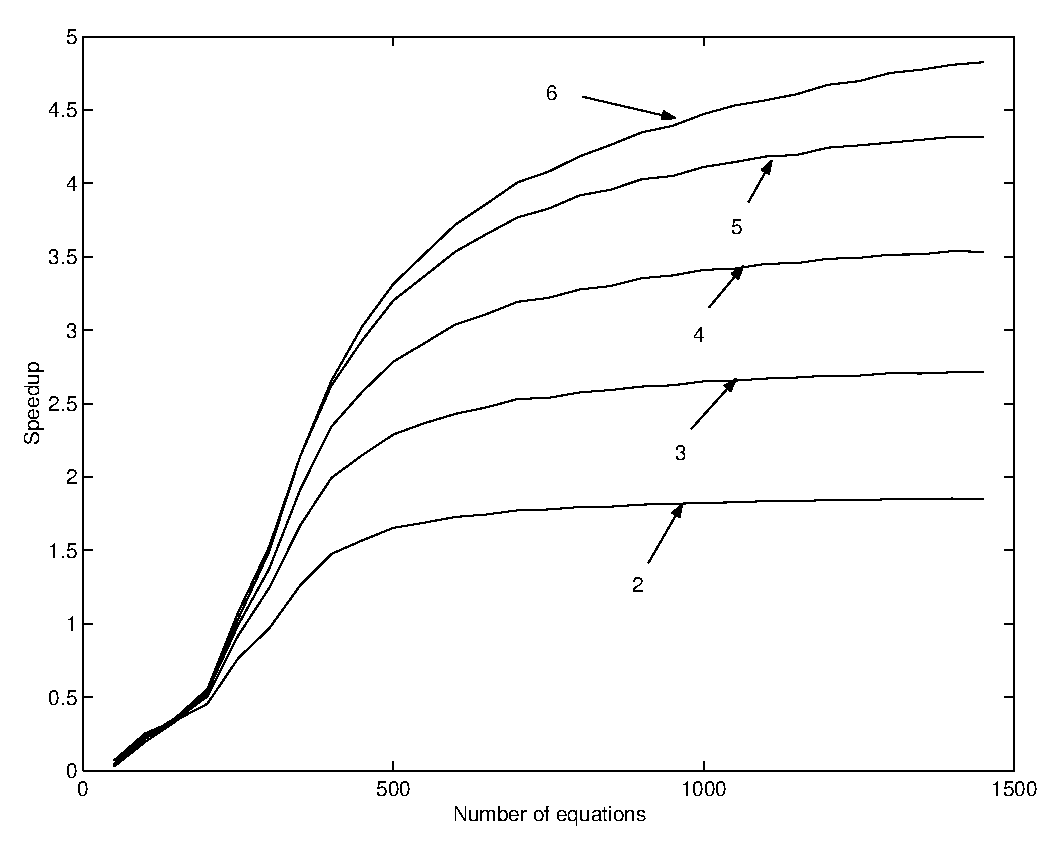
\includegraphics[scale=0.44]{gj-mpich2-bw.eps}
   \caption{Gauss-Jordan Speedup}
\end{figure}

%-------------------------------------------------------------------------
\SubSection{Jacobi with dominant rows}

For the Jacobi the matrix and free term will be distributed among
 machines using a block striped row type. In the following graph we show
 the distribution of the matrix and free term over the network 
compared with the serial time of the Jacobi algorithm.

\begin{figure}[h]
   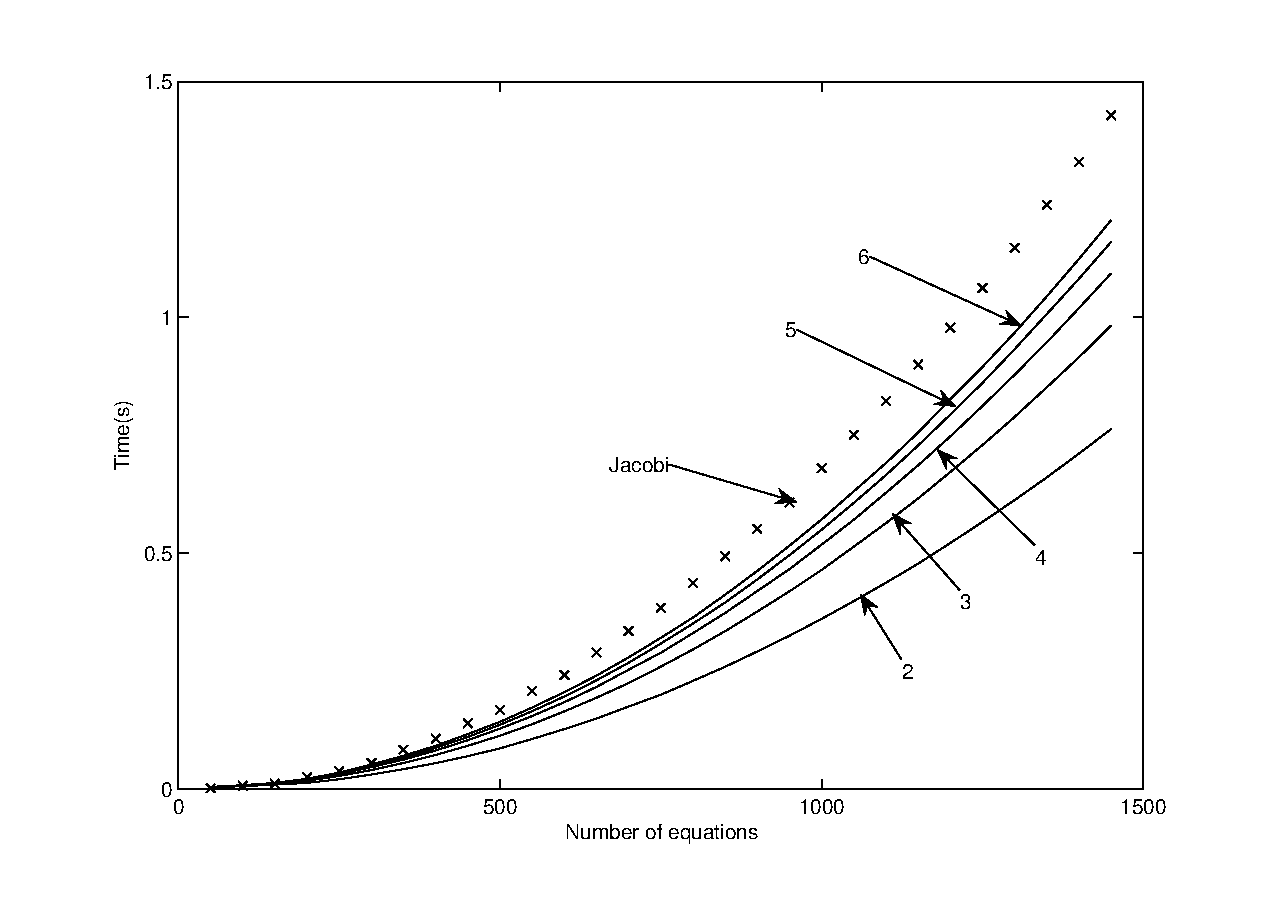
\includegraphics[scale=0.44]{distrib-mpich2-bw.eps}
   \caption{Data distribution}
\end{figure}

With local variable and MPI\_Reduce we compute q using relation \ref{q} and 
$\|x^{(n+1)}-x^{(n)}\|_\infty$  with relation \ref{norma}.We have chosen the block striped row partitioning 
because is the faster way to send a matrix across a network and in one 
iteration Jacobi is not data dependent over rows.
The iteration loop is executed in the block assigned to each machine. 
We compute again $\|x^{(n+1)}-x^{(n)}\|_\infty$.
The result is then concatenated to the fist machine and then with stop condition is broadcasted to 
all machines.

\begin{figure}[h]
   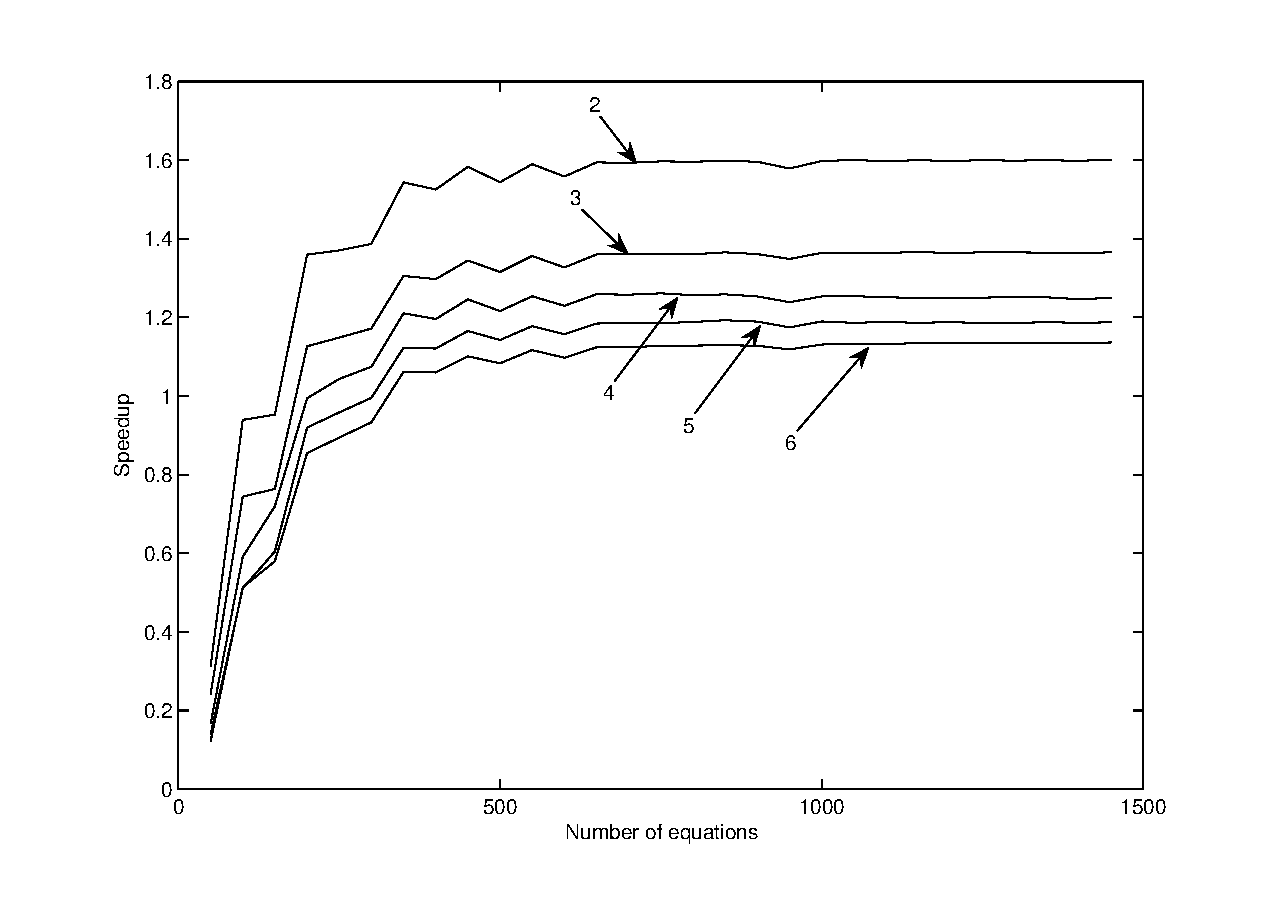
\includegraphics[scale=0.44]{jr-mpich2-bw.eps}
   \caption{Jacobi with dominant rows Speedup}
\end{figure}

%-------------------------------------------------------------------------
\Section{Measurements methodology}

We chose to implement the problems on MPICH2-1.0.2 from Argone
National Laboratory \cite{argone} which is a MPI-2 standard, but
for what we need the MPI-1 standard from MPICH2 is sufficient
because we only use MPI\_Send, MPI\_Recv and MPI\_Bcast and we use
static allocation of resources.

We chose to use the MPI\_Send and MPI\_Recv in favor of MPI\_Isend
and MPI\_Irecv because with blocking function will help us to deal
with synchronization of the machines.

The NOW consists in five Pentium II at 500 MHz with a Realteck
8139 network card connected with a 100Mbs switch. The operating
system is Linux Fedora Core 1 with 2.4.24 kernel.

The linear system is random generated only at startup of the
benchmark and stored in a separate matrix at machine 0. This is
done because Gauss and Gauss-Jordan modifies the matrix.

For the Gauss Elimination and Gauss-Jordan the coefficient matrix
is random generated with uniform distribution. For the Jacobi we
will random generate only the coefficient matrix without the
primary diagonal and the diagonal we will generate with the
relation (\ref{jaccond}).

If we random generate the free term it is a chance that the system
will be not compatible. So we chose the solution
$\{1,2,3,\ldots,n\}$ and with this solution we generate the free
term using the definition of the linear system (\ref{s1}).

Each algorithm is implemented in a function which is finished by
an MPI\_Barrier function.

The time is given using operating system function gettimeofday
before the start of the first distributions and after the tenth
runs. The average time is then save in a file for future analysis.

After the tenth run we verify the correctitude of the solution
with the desired solution $\{1,2,3,\ldots,n\}$.

%-------------------------------------------------------------------------
\Section{Conclusions}

For the Gauss Elimination ang Gauss-Jordan we obtain high speedup for a 
small number of computers but only the computer power is low comparing with 
the network capability, in our case PII at 500MHz to PIII at 800 MHz the 100 MBs network is OK.
But if the power of the computer increses over 800 MHz the limitation of the 
network became very clear and so the speedup decrese to a underunity for PIV
2.4 GHz. If we have a large number of computers or a more powerful processors
we have to update the network to Giganet or Myrinet.

The Jacobi iterative methode, which is low computational, is not
suitable for implementation on low cost distributed cluster
because the data distribution is comparative with the serial time.
And so the speedup is under unity. But if the data is scaterred over
machines the speedup is increased.

%-------------------------------------------------------------------------
\nocite{numerice}
\bibliographystyle{latex8}
\bibliography{cluster}

\end{document}
